\documentclass{article}
\usepackage{amsmath}
\usepackage{amssymb}
\usepackage{amsthm}
\usepackage{graphicx}

\newcommand{\pf}{{Pfaffian~}}
\renewcommand{\a}[1]{a_{#1}}
\newtheorem{theorem}{Theorem}[section]
\newtheorem{algorithm}[theorem]{Algorithm}
\newtheorem{lemma}[theorem]{Lemma}

\newcommand{\A}{\begin{pmatrix}
0 & a_{12} & a_{13} & a_{14} \\
-a_{12} & 0 & a_{23} & a_{24} \\
-a_{13} & -a_{23} & 0 & a_{34} \\
-a_{14} & -a_{24} & -a_{34} & 0
\end{pmatrix}}
\newcommand{\B}{\begin{pmatrix}
a_{15} & a_{16} \\
a_{25} & a_{26} \\
a_{36} & a_{36} \\
a_{45} & a_{46}
\end{pmatrix}}
\newcommand{\C}{
\begin{pmatrix}
-a_{15} & a_{25} & -a_{35} & a_{45} \\
-a_{16} & a_{26} & -a_{36} & a_{46}
\end{pmatrix}}
\newcommand{\D}{
\begin{pmatrix}
0 & a_{56} \\
-a_{56} & 0
\end{pmatrix}}
\author{Rikard Hjort\\\texttt{hjortr@student.chalmers.se}}
\date{today}
\title{\pf matrices}

\begin{document}
\maketitle

\section{Compute the determinant of a $6 \times 6$ skew symetric matrix in which the elements above the diagonal are independent indeterminates over the ring of rational integers}

A skew symmetric matrix is defined as a matrix $M$ for which $M^T = -M$. If $M$
is a $6 \times 6$ matrix, then

\begin{equation*}
M =
\begin{pmatrix}
0 & a_{12} & a_{13} & a_{14} & a_{15} & a_{16} \\
-a_{12} & 0 & a_{23} & a_{24} & a_{25} & a_{26} \\
-a_{13} & -a_{23} & 0 & a_{34} & a_{35} & a_{36} \\
-a_{14} & -a_{24} & -a_{34} & 0 & a_{45} & a_{46} \\
-a_{15} & -a_{25} & -a_{35} & -a_{45} & 0 & a_{56} \\
-a_{16} & -a_{26} & -a_{36} & -a_{46} & -a_{56} & 0
\end{pmatrix}
\end{equation*}

Each element above the diagonal is an integer, and for each element $a_{ij}$
below the diagonal, $a_{ij} = -a_{ji}$. Further, all the elements on the
diagonal are 0, since $a_{ii} = -a_{ii} \Leftarrow 2a_{ii} = 0 \Leftrightarrow
a_{ii} = 0$ for the ring of integers.

To calculate the determinant, we use the fact that if
\begin{equation*}
M =
\begin{pmatrix}
A & B \\
C & D
\end{pmatrix}
\end{equation*}

\noindent and $D$ is singular, then $$\det(M) = \det(D)\det(A - BD^{-1}C)$$

The following lemma will greatly simplify the calculations.

\begin{lemma}\label{square}
  If $M$ is a skew symmetric $4 \times 4$ matrix, then
  $$\det(M) = (\a{12} \a{34} - \a{13} \a{24} + \a{14} \a{23})^2$$ 
\end{lemma}
\begin{proof}
  This follows from developing the determinant in the usual fashion to find that
  \begin{equation*}
    \begin{split}
    \det(M) =& \\
    &(\a{12}\a{34})^2 + (\a{13}\a{24})^2 + (\a{14}\a{23})^2 \\
    &- 2\a{12}\a{13}\a{24}\a{34} + 2\a{12}\a{14}\a{23}\a{34} - 2 \a{13}\a{14}\a{23}\a{24}\\
    =&\;(\a{12} \a{34} - \a{13} \a{24} + \a{14} \a{23})^2
    \end{split}
\end{equation*}
\end{proof}

Now set

\begin{equation*}
\begin{split}
A = \A
B = &\B\\
C = \C
D = &\D
\end{split}
\end{equation*}

We now begin calculating $\det(D)\det(A - BD^{-1}C)$. First,
\begin{equation}\label{det_D}
  \det(D) = \a{56}^2
\end{equation}
We proceed with $A - BD^{-1}C$. However, we will first note that $A$ is
skew symmetric. It will so happen that $BD^{-1}C$ is also skew symmetric, so $A
- BD^{-1}C$ is skew symmetric, too, and $4 \times 4$, so we can make use of
lemma \ref{square} to calculate $\det(A - BD^{-1}C)$.

\begin{equation*}
  \begin{split}
D^{-1} &=
\begin{pmatrix}
0 & -\frac{1}{a_{56}} \\
\frac{1}{a_{56}} & 0
\end{pmatrix}
\end{split}
\end{equation*}

We can note immediately that this means the only valid value of $a_{56}$ is 1
and $-1$. For any other value, $a_{56}$ lacks a multiplicative inverse in the
ring of integers. We will continue to use $\frac{1}{a_{56}}$ for generality, but one may
note the calculations can be somewhat simplified by setting it to $a_{56}$
directly, as 1 and $-1$ are their own inverses.\footnote{How does this affect a
  general matrix over the ring of integers? Well, it hurts generalizability. But
since we will be working with skew symmetric \textit{adjacency} matrices, we can
accept elements being restrained to -1 and 1. For a more general solution, we
would use the definitition $\det(M) = \sum_{\sigma \in
  S_n}sgn(\sigma)\prod_{i=1}^na_{i,\sigma(i)})$, and solve from there.}
\begin{equation}\label{abdinvc}
  \begin{split}
BD^{-1}C &=
\B
D^{-1}
\C
\\
&= \frac{1}{\a{56}}(\a{i5}\a{j6} - \a{i6}\a{j5})
\\
A - BD^{-1}C &= (\a{ij} - \frac{1}{\a{56}} ( \a{i5}\a{j6} - \a{i6}\a{j5}))\\
&= \frac{1}{\a{56}}(\a{ij}\a{56} - \a{i5}\a{j6} + \a{i6}\a{j5})\\
\text{ for every }& 1 \leq i < j \leq 4
\end{split}
\end{equation}

Note in equation (\ref{abdinvc}) that for $i = j$ the entry is 0, and for $-i, -j$
the entry is the negative of that for $i, j$, so $BD^{-1}C$ is
a skew symmetric matrix.

We are now ready to use lemma \ref{square} to compute the determinant. We simply
replace $i$ and $j$ in the result of equation (\ref{abdinvc}) with the row and
column numbers in the lemma.

\begin{equation}
  \begin{split}
    \det(M) = &\det(D)\det(A - BD^{-1}C) \\
   = \a{56}^2(
            &\frac{1}{\a{56}}(\a{12}\a{56} - \a{15}\a{26} + \a{16}\a{25}) \frac{1}{\a{56}}(\a{34}\a{56} - \a{35}\a{46} + \a{36}\a{45}) \\% (1 2)(3 4)
          - &\frac{1}{\a{56}}(\a{13}\a{56} - \a{15}\a{36} + \a{16}\a{35}) \frac{1}{\a{56}}(\a{24}\a{56} - \a{25}\a{46} + \a{26}\a{45}) \\% (1 3)(2 4)
          + &\frac{1}{\a{56}}(\a{14}\a{56} - \a{15}\a{46} + \a{16}\a{45}) \frac{1}{\a{56}}(\a{23}\a{56} - \a{25}\a{36} + \a{26}\a{35}) % (1 4)(2 3)
          )^2\\
%   = \a{56}^2(\frac{1}{\a{56}^2} 
%            &((\a{12}\a{56} - \a{15}\a{26} + \a{16}\a{25}) (\a{34}\a{56} - \a{35}\a{46} + \a{36}\a{45}) \\% (1 2)(3 4)
%          - &(\a{13}\a{56} - \a{15}\a{36} + \a{16}\a{35}) (\a{24}\a{56} - \a{25}\a{46} + \a{26}\a{45}) \\% (1 3)(2 4)
%          + &(\a{14}\a{56} - \a{15}\a{46} + \a{16}\a{45}) (\a{23}\a{56} - \a{25}\a{36} + \a{26}\a{35}) % (1 4)(2 3)
%          ))^2\\
   = \frac{1}{\a{56}^2}(
            &(\a{12}\a{56} - \a{15}\a{26} + \a{16}\a{25}) (\a{34}\a{56} - \a{35}\a{46} + \a{36}\a{45}) \\
          - &(\a{13}\a{56} - \a{15}\a{36} + \a{16}\a{35}) (\a{24}\a{56} - \a{25}\a{46} + \a{26}\a{45}) \\
          + &(\a{14}\a{56} - \a{15}\a{46} + \a{16}\a{45}) (\a{23}\a{56} - \a{25}\a{36} + \a{26}\a{35})
          )^2\\
  \end{split}
  \end{equation}
    %=&\;(\a{12} \a{34} - \a{13} \a{24} + \a{14} \a{23})^2

By a final simplification, due to the note earlier about $\frac{1}{a_{56}} =
a_{56} = \pm 1$, we get

\begin{equation}
  \begin{split}
    \det(M) =  \\
   = (
            &(\a{12}\a{56} - \a{15}\a{26} + \a{16}\a{25}) (\a{34}\a{56} - \a{35}\a{46} + \a{36}\a{45}) \\
          - &(\a{13}\a{56} - \a{15}\a{36} + \a{16}\a{35}) (\a{24}\a{56} - \a{25}\a{46} + \a{26}\a{45}) \\
          + &(\a{14}\a{56} - \a{15}\a{46} + \a{16}\a{45}) (\a{23}\a{56} - \a{25}\a{36} + \a{26}\a{35})
          )^2
  \end{split}
  \end{equation}

\section{Discuss its relation with all the perfect matchings of complete graph $K_6$}

By looking at equation (\ref{abdinvc}), we can see that every term of

$$
A - BD^{-1}C &= \pm(\a{ij}\a{56} - \a{i5}\a{j6} + \a{i6}\a{j5}) \text{\quad for
  all } 1 \leq i < j \leq 4
$$

We may note that each of the three terms in in every element represents one way
to combine $i, j$ with $5,6$. Thus, in terms of matchings, we may interpret each
term as picking two edges in $K_6$. We may also note that for every term, it is
not possible to pick $i,j$ such that any of the edges share a vertix. This means
that after picking these two edges, exactly 4 vertices have a picked edge into
them, meaning two vertices remain, and by picking the dege between those two we
obtain a perfect matching. 

Thus, above $4\times4$ matrix enumerates all perfect matching in an interesting
way. Each element not on the diagonal enumerates 3 matchings, with repetition
under and over the diagonal. So there are $6$ ``unique'' sets of matchings,
giving a total of 18 matchings. However, among these, there will be 3
duplicates (when we pick the edges \{5, 6\} and then $\{i, j\}$, this is
identical to picking $\{5, 6\}$ and $\{1, 2, 3, 4\} \backslash \{5,6, i, j\}$),
and thus we have 15 perfect matchings. We can easily check that this is the
correct number, by its correspondence with
$$\frac{\binom{6}{2}\binom{4}{2}\binom{2}{2}}{3!} = 15$$

\paragraph{Closing notes} I suspect that using the formula
$$\det(M) = \sum_{\sigma \in S_n}sgn(\sigma)\prod_{i=1}^na_{i,\sigma(i)})$$

\noindent might have yielded more rewarding results, perhaps a polynomial
directly containing the desired monomials representing the perfect matchings.

% Use Tutte's theorem, and the fact that the determinant is an expression that
% gives you perfect matchings.

% By Cayley's theorem, for an $n\times n$ graph with $n$ even,
% $$\det(M) = Pf(M)^2$$
% 
% where $Pf(M)$ is the Pfaffian of $M$. The determinant of the $K_6$ is easily
% calculated with the formula above: since every $a_{ij} = 1$, all the products
% are 1, and
% $$\det{K_6} = (1\cdot 1 - 1 \cdot 1 + 1 \cdot 1)^2 = 1$$

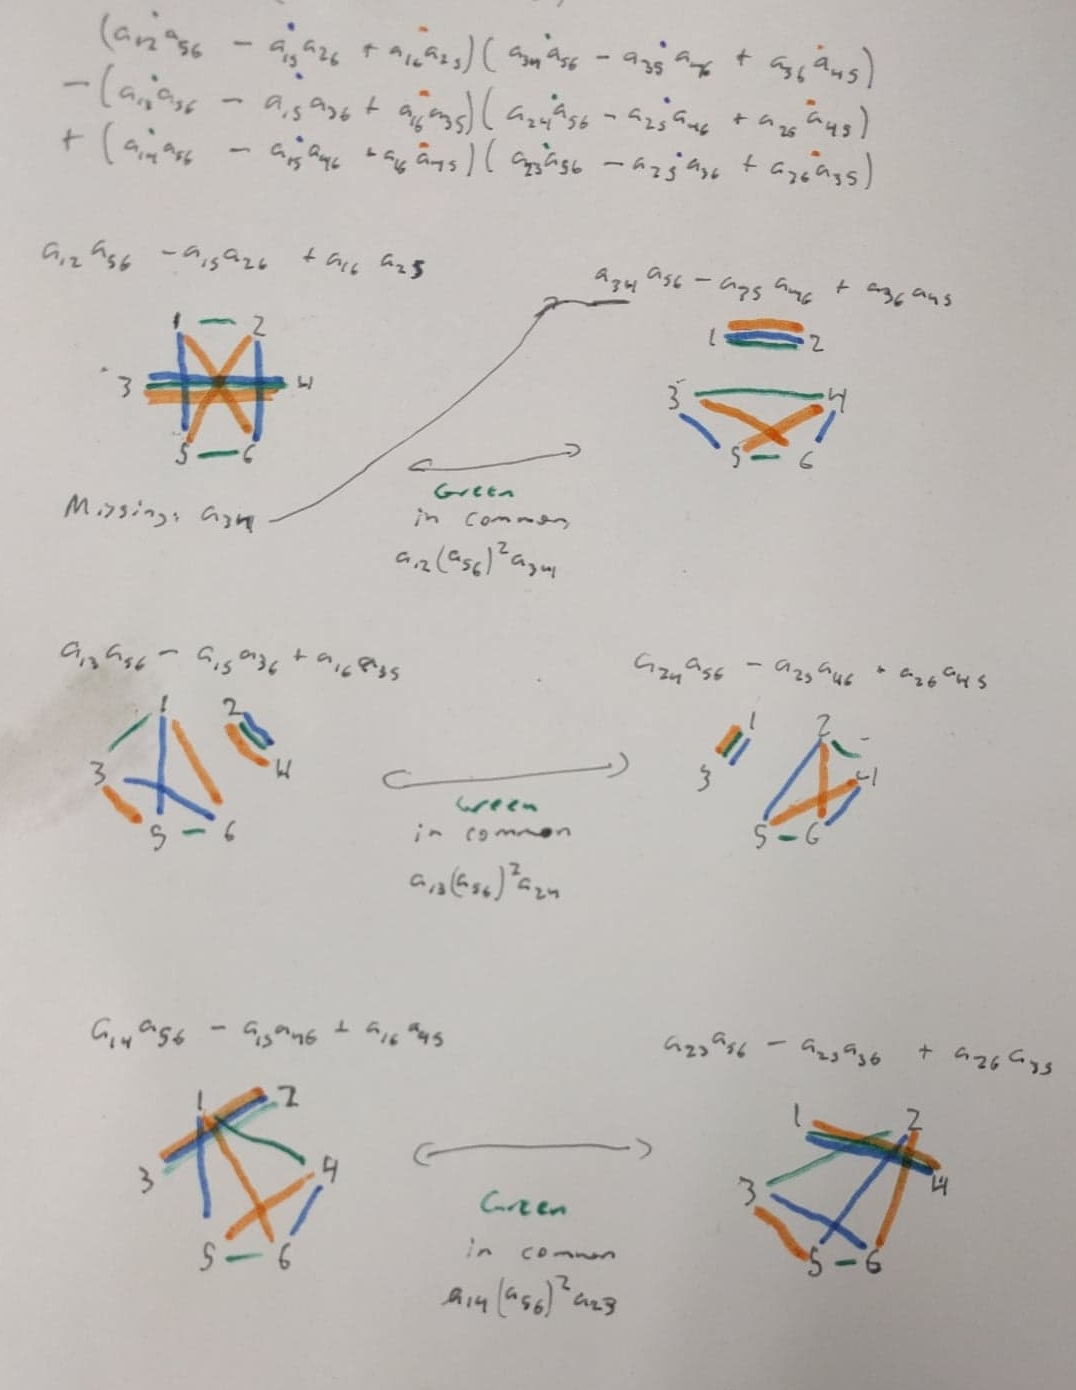
\includegraphics[width=\textwidth]{MatchingsEnumerated}
\end{document}